\documentclass[twoside]{book}

% Packages required by doxygen
\usepackage{fixltx2e}
\usepackage{calc}
\usepackage{doxygen}
\usepackage[export]{adjustbox} % also loads graphicx
\usepackage{graphicx}
\usepackage[utf8]{inputenc}
\usepackage{makeidx}
\usepackage{multicol}
\usepackage{multirow}
\PassOptionsToPackage{warn}{textcomp}
\usepackage{textcomp}
\usepackage[nointegrals]{wasysym}
\usepackage[table]{xcolor}

% Font selection
\usepackage[T1]{fontenc}
\usepackage[scaled=.90]{helvet}
\usepackage{courier}
\usepackage{amssymb}
\usepackage{sectsty}
\renewcommand{\familydefault}{\sfdefault}
\allsectionsfont{%
  \fontseries{bc}\selectfont%
  \color{darkgray}%
}
\renewcommand{\DoxyLabelFont}{%
  \fontseries{bc}\selectfont%
  \color{darkgray}%
}
\newcommand{\+}{\discretionary{\mbox{\scriptsize$\hookleftarrow$}}{}{}}

% Page & text layout
\usepackage{geometry}
\geometry{%
  a4paper,%
  top=2.5cm,%
  bottom=2.5cm,%
  left=2.5cm,%
  right=2.5cm%
}
\tolerance=750
\hfuzz=15pt
\hbadness=750
\setlength{\emergencystretch}{15pt}
\setlength{\parindent}{0cm}
\setlength{\parskip}{3ex plus 2ex minus 2ex}
\makeatletter
\renewcommand{\paragraph}{%
  \@startsection{paragraph}{4}{0ex}{-1.0ex}{1.0ex}{%
    \normalfont\normalsize\bfseries\SS@parafont%
  }%
}
\renewcommand{\subparagraph}{%
  \@startsection{subparagraph}{5}{0ex}{-1.0ex}{1.0ex}{%
    \normalfont\normalsize\bfseries\SS@subparafont%
  }%
}
\makeatother

% Headers & footers
\usepackage{fancyhdr}
\pagestyle{fancyplain}
\fancyhead[LE]{\fancyplain{}{\bfseries\thepage}}
\fancyhead[CE]{\fancyplain{}{}}
\fancyhead[RE]{\fancyplain{}{\bfseries\leftmark}}
\fancyhead[LO]{\fancyplain{}{\bfseries\rightmark}}
\fancyhead[CO]{\fancyplain{}{}}
\fancyhead[RO]{\fancyplain{}{\bfseries\thepage}}
\fancyfoot[LE]{\fancyplain{}{}}
\fancyfoot[CE]{\fancyplain{}{}}
\fancyfoot[RE]{\fancyplain{}{\bfseries\scriptsize Generated by Doxygen }}
\fancyfoot[LO]{\fancyplain{}{\bfseries\scriptsize Generated by Doxygen }}
\fancyfoot[CO]{\fancyplain{}{}}
\fancyfoot[RO]{\fancyplain{}{}}
\renewcommand{\footrulewidth}{0.4pt}
\renewcommand{\chaptermark}[1]{%
  \markboth{#1}{}%
}
\renewcommand{\sectionmark}[1]{%
  \markright{\thesection\ #1}%
}

% Indices & bibliography
\usepackage{natbib}
\usepackage[titles]{tocloft}
\setcounter{tocdepth}{3}
\setcounter{secnumdepth}{5}
\makeindex

% Hyperlinks (required, but should be loaded last)
\usepackage{ifpdf}
\ifpdf
  \usepackage[pdftex,pagebackref=true]{hyperref}
\else
  \usepackage[ps2pdf,pagebackref=true]{hyperref}
\fi
\hypersetup{%
  colorlinks=true,%
  linkcolor=blue,%
  citecolor=blue,%
  unicode%
}

% Custom commands
\newcommand{\clearemptydoublepage}{%
  \newpage{\pagestyle{empty}\cleardoublepage}%
}

\usepackage{caption}
\captionsetup{labelsep=space,justification=centering,font={bf},singlelinecheck=off,skip=4pt,position=top}

%===== C O N T E N T S =====

\begin{document}

% Titlepage & ToC
\hypersetup{pageanchor=false,
             bookmarksnumbered=true,
             pdfencoding=unicode
            }
\pagenumbering{alph}
\begin{titlepage}
\vspace*{7cm}
\begin{center}%
{\Large Mantenimiento Clientes \\[1ex]\large 0.\+0.\+1 }\\
\vspace*{1cm}
{\large Generated by Doxygen 1.8.14}\\
\end{center}
\end{titlepage}
\clearemptydoublepage
\pagenumbering{roman}
\tableofcontents
\clearemptydoublepage
\pagenumbering{arabic}
\hypersetup{pageanchor=true}

%--- Begin generated contents ---
\chapter{Namespace Index}
\section{Packages}
Here are the packages with brief descriptions (if available)\+:\begin{DoxyCompactList}
\item\contentsline{section}{\mbox{\hyperlink{namespace_ejem___mantenimiento___personas}{Ejem\+\_\+\+Mantenimiento\+\_\+\+Personas}} }{\pageref{namespace_ejem___mantenimiento___personas}}{}
\end{DoxyCompactList}

\chapter{Hierarchical Index}
\section{Class Hierarchy}
This inheritance list is sorted roughly, but not completely, alphabetically\+:\begin{DoxyCompactList}
\item \contentsline{section}{Ejem\+\_\+\+Mantenimiento\+\_\+\+Personas.\+Cliente}{\pageref{class_ejem___mantenimiento___personas_1_1_cliente}}{}
\item \contentsline{section}{Ejem\+\_\+\+Mantenimiento\+\_\+\+Personas.\+Conexion}{\pageref{class_ejem___mantenimiento___personas_1_1_conexion}}{}
\item Form\begin{DoxyCompactList}
\item \contentsline{section}{Ejem\+\_\+\+Mantenimiento\+\_\+\+Personas.\+Mantenimiento\+Cliente}{\pageref{class_ejem___mantenimiento___personas_1_1_mantenimiento_cliente}}{}
\end{DoxyCompactList}
\end{DoxyCompactList}

\chapter{Class Index}
\section{Class List}
Here are the classes, structs, unions and interfaces with brief descriptions\+:\begin{DoxyCompactList}
\item\contentsline{section}{\mbox{\hyperlink{class_ejem___mantenimiento___personas_1_1_cliente}{Ejem\+\_\+\+Mantenimiento\+\_\+\+Personas.\+Cliente}} \\*Classe \mbox{\hyperlink{class_ejem___mantenimiento___personas_1_1_cliente}{Cliente}}\+: Modelo de datos para los clientes. }{\pageref{class_ejem___mantenimiento___personas_1_1_cliente}}{}
\item\contentsline{section}{\mbox{\hyperlink{class_ejem___mantenimiento___personas_1_1_conexion}{Ejem\+\_\+\+Mantenimiento\+\_\+\+Personas.\+Conexion}} \\*Class \mbox{\hyperlink{class_ejem___mantenimiento___personas_1_1_conexion}{Conexion}}. Gestiona la conexion y transferencia de datos a la base de datos. }{\pageref{class_ejem___mantenimiento___personas_1_1_conexion}}{}
\item\contentsline{section}{\mbox{\hyperlink{class_ejem___mantenimiento___personas_1_1_mantenimiento_cliente}{Ejem\+\_\+\+Mantenimiento\+\_\+\+Personas.\+Mantenimiento\+Cliente}} \\*Formulario de mantenimiento para los clientes. }{\pageref{class_ejem___mantenimiento___personas_1_1_mantenimiento_cliente}}{}
\end{DoxyCompactList}

\chapter{Namespace Documentation}
\hypertarget{namespace_ejem___mantenimiento___personas}{}\section{Ejem\+\_\+\+Mantenimiento\+\_\+\+Personas Namespace Reference}
\label{namespace_ejem___mantenimiento___personas}\index{Ejem\+\_\+\+Mantenimiento\+\_\+\+Personas@{Ejem\+\_\+\+Mantenimiento\+\_\+\+Personas}}
\subsection*{Classes}
\begin{DoxyCompactItemize}
\item 
class \mbox{\hyperlink{class_ejem___mantenimiento___personas_1_1_cliente}{Cliente}}
\begin{DoxyCompactList}\small\item\em Classe \mbox{\hyperlink{class_ejem___mantenimiento___personas_1_1_cliente}{Cliente}}\+: Modelo de datos para los clientes. \end{DoxyCompactList}\item 
class \mbox{\hyperlink{class_ejem___mantenimiento___personas_1_1_conexion}{Conexion}}
\begin{DoxyCompactList}\small\item\em Class \mbox{\hyperlink{class_ejem___mantenimiento___personas_1_1_conexion}{Conexion}}. Gestiona la conexion y transferencia de datos a la base de datos. \end{DoxyCompactList}\item 
class \mbox{\hyperlink{class_ejem___mantenimiento___personas_1_1_mantenimiento_cliente}{Mantenimiento\+Cliente}}
\begin{DoxyCompactList}\small\item\em Formulario de mantenimiento para los clientes. \end{DoxyCompactList}\item 
class {\bfseries Program}
\end{DoxyCompactItemize}

\chapter{Class Documentation}
\hypertarget{class_ejem___mantenimiento___personas_1_1_cliente}{}\section{Ejem\+\_\+\+Mantenimiento\+\_\+\+Personas.\+Cliente Class Reference}
\label{class_ejem___mantenimiento___personas_1_1_cliente}\index{Ejem\+\_\+\+Mantenimiento\+\_\+\+Personas.\+Cliente@{Ejem\+\_\+\+Mantenimiento\+\_\+\+Personas.\+Cliente}}


Classe \mbox{\hyperlink{class_ejem___mantenimiento___personas_1_1_cliente}{Cliente}}\+: Modelo de datos para los clientes.  




Collaboration diagram for Ejem\+\_\+\+Mantenimiento\+\_\+\+Personas.\+Cliente\+:
\nopagebreak
\begin{figure}[H]
\begin{center}
\leavevmode
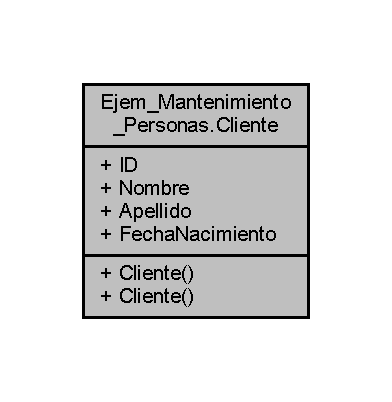
\includegraphics[width=188pt]{class_ejem___mantenimiento___personas_1_1_cliente__coll__graph}
\end{center}
\end{figure}
\subsection*{Public Member Functions}
\begin{DoxyCompactItemize}
\item 
\mbox{\hyperlink{class_ejem___mantenimiento___personas_1_1_cliente_a6df93124462da1bb67a5274db3d7a2d4}{Cliente}} ()
\begin{DoxyCompactList}\small\item\em Constructor sin parametros para la clase cliente. \end{DoxyCompactList}\item 
\mbox{\hyperlink{class_ejem___mantenimiento___personas_1_1_cliente_aa963edf25ca30a5fd262340cb3046d61}{Cliente}} (string nombre, string apellido, string fecha\+Nacimiento)
\begin{DoxyCompactList}\small\item\em Constructor(); con parametros para la clase cliente. \end{DoxyCompactList}\end{DoxyCompactItemize}
\subsection*{Properties}
\begin{DoxyCompactItemize}
\item 
int \mbox{\hyperlink{class_ejem___mantenimiento___personas_1_1_cliente_ae229bd0285e992ec0170c930ea508dc6}{ID}}\hspace{0.3cm}{\ttfamily  \mbox{[}get, set\mbox{]}}
\begin{DoxyCompactList}\small\item\em Setter y Getter para el atributo int ID del cliente. \end{DoxyCompactList}\item 
string \mbox{\hyperlink{class_ejem___mantenimiento___personas_1_1_cliente_abfd662cc9b3f46750983780c39dc6aef}{Nombre}}\hspace{0.3cm}{\ttfamily  \mbox{[}get, set\mbox{]}}
\begin{DoxyCompactList}\small\item\em Setter y Getter para el atributo string Nombre del cliente. \end{DoxyCompactList}\item 
string \mbox{\hyperlink{class_ejem___mantenimiento___personas_1_1_cliente_ac0182fb39e68117ec4aa6a35902d4f26}{Apellido}}\hspace{0.3cm}{\ttfamily  \mbox{[}get, set\mbox{]}}
\begin{DoxyCompactList}\small\item\em Setter y Getter para el atributo string Apellido del cliente. \end{DoxyCompactList}\item 
string \mbox{\hyperlink{class_ejem___mantenimiento___personas_1_1_cliente_a7c8f3f7bd7733225040113148b71884e}{Fecha\+Nacimiento}}\hspace{0.3cm}{\ttfamily  \mbox{[}get, set\mbox{]}}
\begin{DoxyCompactList}\small\item\em Setter y Getter para el atributo string Fecha\+Nacimiento del cliente. \end{DoxyCompactList}\end{DoxyCompactItemize}


\subsection{Detailed Description}
Classe \mbox{\hyperlink{class_ejem___mantenimiento___personas_1_1_cliente}{Cliente}}\+: Modelo de datos para los clientes. 



\subsection{Constructor \& Destructor Documentation}
\mbox{\Hypertarget{class_ejem___mantenimiento___personas_1_1_cliente_a6df93124462da1bb67a5274db3d7a2d4}\label{class_ejem___mantenimiento___personas_1_1_cliente_a6df93124462da1bb67a5274db3d7a2d4}} 
\index{Ejem\+\_\+\+Mantenimiento\+\_\+\+Personas\+::\+Cliente@{Ejem\+\_\+\+Mantenimiento\+\_\+\+Personas\+::\+Cliente}!Cliente@{Cliente}}
\index{Cliente@{Cliente}!Ejem\+\_\+\+Mantenimiento\+\_\+\+Personas\+::\+Cliente@{Ejem\+\_\+\+Mantenimiento\+\_\+\+Personas\+::\+Cliente}}
\subsubsection{\texorpdfstring{Cliente()}{Cliente()}\hspace{0.1cm}{\footnotesize\ttfamily [1/2]}}
{\footnotesize\ttfamily Ejem\+\_\+\+Mantenimiento\+\_\+\+Personas.\+Cliente.\+Cliente (\begin{DoxyParamCaption}{ }\end{DoxyParamCaption})}



Constructor sin parametros para la clase cliente. 

\mbox{\Hypertarget{class_ejem___mantenimiento___personas_1_1_cliente_aa963edf25ca30a5fd262340cb3046d61}\label{class_ejem___mantenimiento___personas_1_1_cliente_aa963edf25ca30a5fd262340cb3046d61}} 
\index{Ejem\+\_\+\+Mantenimiento\+\_\+\+Personas\+::\+Cliente@{Ejem\+\_\+\+Mantenimiento\+\_\+\+Personas\+::\+Cliente}!Cliente@{Cliente}}
\index{Cliente@{Cliente}!Ejem\+\_\+\+Mantenimiento\+\_\+\+Personas\+::\+Cliente@{Ejem\+\_\+\+Mantenimiento\+\_\+\+Personas\+::\+Cliente}}
\subsubsection{\texorpdfstring{Cliente()}{Cliente()}\hspace{0.1cm}{\footnotesize\ttfamily [2/2]}}
{\footnotesize\ttfamily Ejem\+\_\+\+Mantenimiento\+\_\+\+Personas.\+Cliente.\+Cliente (\begin{DoxyParamCaption}\item[{string}]{nombre,  }\item[{string}]{apellido,  }\item[{string}]{fecha\+Nacimiento }\end{DoxyParamCaption})}



Constructor(); con parametros para la clase cliente. 


\begin{DoxyParams}{Parameters}
{\em nombre} & String Nombre\+: Nombre del cliente.\\
\hline
{\em apellido} & String Apellido\+: Apellido del cliente.\\
\hline
{\em fecha\+Nacimiento} & String Fecha\+Nacimiento\+: Fecha de nacimiento del cliente.\\
\hline
\end{DoxyParams}


\subsection{Property Documentation}
\mbox{\Hypertarget{class_ejem___mantenimiento___personas_1_1_cliente_ac0182fb39e68117ec4aa6a35902d4f26}\label{class_ejem___mantenimiento___personas_1_1_cliente_ac0182fb39e68117ec4aa6a35902d4f26}} 
\index{Ejem\+\_\+\+Mantenimiento\+\_\+\+Personas\+::\+Cliente@{Ejem\+\_\+\+Mantenimiento\+\_\+\+Personas\+::\+Cliente}!Apellido@{Apellido}}
\index{Apellido@{Apellido}!Ejem\+\_\+\+Mantenimiento\+\_\+\+Personas\+::\+Cliente@{Ejem\+\_\+\+Mantenimiento\+\_\+\+Personas\+::\+Cliente}}
\subsubsection{\texorpdfstring{Apellido}{Apellido}}
{\footnotesize\ttfamily string Ejem\+\_\+\+Mantenimiento\+\_\+\+Personas.\+Cliente.\+Apellido\hspace{0.3cm}{\ttfamily [get]}, {\ttfamily [set]}}



Setter y Getter para el atributo string Apellido del cliente. 

\mbox{\Hypertarget{class_ejem___mantenimiento___personas_1_1_cliente_a7c8f3f7bd7733225040113148b71884e}\label{class_ejem___mantenimiento___personas_1_1_cliente_a7c8f3f7bd7733225040113148b71884e}} 
\index{Ejem\+\_\+\+Mantenimiento\+\_\+\+Personas\+::\+Cliente@{Ejem\+\_\+\+Mantenimiento\+\_\+\+Personas\+::\+Cliente}!Fecha\+Nacimiento@{Fecha\+Nacimiento}}
\index{Fecha\+Nacimiento@{Fecha\+Nacimiento}!Ejem\+\_\+\+Mantenimiento\+\_\+\+Personas\+::\+Cliente@{Ejem\+\_\+\+Mantenimiento\+\_\+\+Personas\+::\+Cliente}}
\subsubsection{\texorpdfstring{Fecha\+Nacimiento}{FechaNacimiento}}
{\footnotesize\ttfamily string Ejem\+\_\+\+Mantenimiento\+\_\+\+Personas.\+Cliente.\+Fecha\+Nacimiento\hspace{0.3cm}{\ttfamily [get]}, {\ttfamily [set]}}



Setter y Getter para el atributo string Fecha\+Nacimiento del cliente. 

\mbox{\Hypertarget{class_ejem___mantenimiento___personas_1_1_cliente_ae229bd0285e992ec0170c930ea508dc6}\label{class_ejem___mantenimiento___personas_1_1_cliente_ae229bd0285e992ec0170c930ea508dc6}} 
\index{Ejem\+\_\+\+Mantenimiento\+\_\+\+Personas\+::\+Cliente@{Ejem\+\_\+\+Mantenimiento\+\_\+\+Personas\+::\+Cliente}!ID@{ID}}
\index{ID@{ID}!Ejem\+\_\+\+Mantenimiento\+\_\+\+Personas\+::\+Cliente@{Ejem\+\_\+\+Mantenimiento\+\_\+\+Personas\+::\+Cliente}}
\subsubsection{\texorpdfstring{ID}{ID}}
{\footnotesize\ttfamily int Ejem\+\_\+\+Mantenimiento\+\_\+\+Personas.\+Cliente.\+ID\hspace{0.3cm}{\ttfamily [get]}, {\ttfamily [set]}}



Setter y Getter para el atributo int ID del cliente. 

\mbox{\Hypertarget{class_ejem___mantenimiento___personas_1_1_cliente_abfd662cc9b3f46750983780c39dc6aef}\label{class_ejem___mantenimiento___personas_1_1_cliente_abfd662cc9b3f46750983780c39dc6aef}} 
\index{Ejem\+\_\+\+Mantenimiento\+\_\+\+Personas\+::\+Cliente@{Ejem\+\_\+\+Mantenimiento\+\_\+\+Personas\+::\+Cliente}!Nombre@{Nombre}}
\index{Nombre@{Nombre}!Ejem\+\_\+\+Mantenimiento\+\_\+\+Personas\+::\+Cliente@{Ejem\+\_\+\+Mantenimiento\+\_\+\+Personas\+::\+Cliente}}
\subsubsection{\texorpdfstring{Nombre}{Nombre}}
{\footnotesize\ttfamily string Ejem\+\_\+\+Mantenimiento\+\_\+\+Personas.\+Cliente.\+Nombre\hspace{0.3cm}{\ttfamily [get]}, {\ttfamily [set]}}



Setter y Getter para el atributo string Nombre del cliente. 



The documentation for this class was generated from the following file\+:\begin{DoxyCompactItemize}
\item 
Cliente.\+cs\end{DoxyCompactItemize}

\hypertarget{class_ejem___mantenimiento___personas_1_1_conexion}{}\section{Ejem\+\_\+\+Mantenimiento\+\_\+\+Personas.\+Conexion Class Reference}
\label{class_ejem___mantenimiento___personas_1_1_conexion}\index{Ejem\+\_\+\+Mantenimiento\+\_\+\+Personas.\+Conexion@{Ejem\+\_\+\+Mantenimiento\+\_\+\+Personas.\+Conexion}}


Class \mbox{\hyperlink{class_ejem___mantenimiento___personas_1_1_conexion}{Conexion}}. Gestiona la conexion y transferencia de datos a la base de datos.  




Collaboration diagram for Ejem\+\_\+\+Mantenimiento\+\_\+\+Personas.\+Conexion\+:
\nopagebreak
\begin{figure}[H]
\begin{center}
\leavevmode
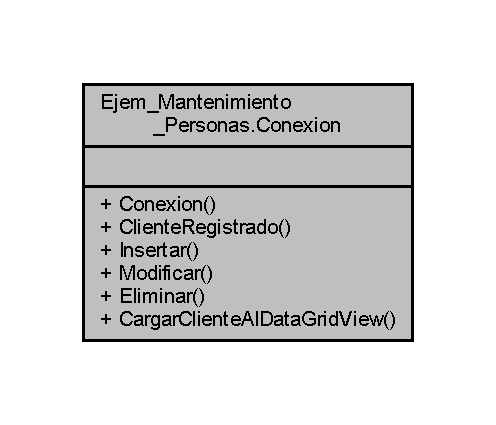
\includegraphics[width=238pt]{class_ejem___mantenimiento___personas_1_1_conexion__coll__graph}
\end{center}
\end{figure}
\subsection*{Public Member Functions}
\begin{DoxyCompactItemize}
\item 
bool \mbox{\hyperlink{class_ejem___mantenimiento___personas_1_1_conexion_a6eb70e84b86424966c75d5859d241a40}{Cliente\+Registrado}} (int id)
\begin{DoxyCompactList}\small\item\em Verifica la existencia de un cliente en la base de datos. \end{DoxyCompactList}\item 
string \mbox{\hyperlink{class_ejem___mantenimiento___personas_1_1_conexion_a8f2099b092af61b02fa7b96c491fe1f5}{Insertar}} (\mbox{\hyperlink{class_ejem___mantenimiento___personas_1_1_cliente}{Cliente}} cli)
\begin{DoxyCompactList}\small\item\em Agrega un cliente a la base de datos. \end{DoxyCompactList}\item 
string \mbox{\hyperlink{class_ejem___mantenimiento___personas_1_1_conexion_a1fc3cac8eff1c8f2f7197b56e7209df6}{Modificar}} (\mbox{\hyperlink{class_ejem___mantenimiento___personas_1_1_cliente}{Cliente}} cli)
\begin{DoxyCompactList}\small\item\em Actualiza el registro del cliente, en la base de datos. \end{DoxyCompactList}\item 
string \mbox{\hyperlink{class_ejem___mantenimiento___personas_1_1_conexion_a97b8be1c8c50cfb4d2f0babd96567262}{Eliminar}} (int id)
\begin{DoxyCompactList}\small\item\em Elimina el cliente seleccionado de la base de datos. \end{DoxyCompactList}\item 
void \mbox{\hyperlink{class_ejem___mantenimiento___personas_1_1_conexion_a7907319c7bc72f21b509cc5812b5896c}{Cargar\+Cliente\+Al\+Data\+Grid\+View}} (Data\+Grid\+View data\+Drid\+View)
\begin{DoxyCompactList}\small\item\em Carga la lista de clientes de la base de datos al Data\+Grid\+View. \end{DoxyCompactList}\end{DoxyCompactItemize}


\subsection{Detailed Description}
Class \mbox{\hyperlink{class_ejem___mantenimiento___personas_1_1_conexion}{Conexion}}. Gestiona la conexion y transferencia de datos a la base de datos. 



\subsection{Member Function Documentation}
\mbox{\Hypertarget{class_ejem___mantenimiento___personas_1_1_conexion_a7907319c7bc72f21b509cc5812b5896c}\label{class_ejem___mantenimiento___personas_1_1_conexion_a7907319c7bc72f21b509cc5812b5896c}} 
\index{Ejem\+\_\+\+Mantenimiento\+\_\+\+Personas\+::\+Conexion@{Ejem\+\_\+\+Mantenimiento\+\_\+\+Personas\+::\+Conexion}!Cargar\+Cliente\+Al\+Data\+Grid\+View@{Cargar\+Cliente\+Al\+Data\+Grid\+View}}
\index{Cargar\+Cliente\+Al\+Data\+Grid\+View@{Cargar\+Cliente\+Al\+Data\+Grid\+View}!Ejem\+\_\+\+Mantenimiento\+\_\+\+Personas\+::\+Conexion@{Ejem\+\_\+\+Mantenimiento\+\_\+\+Personas\+::\+Conexion}}
\subsubsection{\texorpdfstring{Cargar\+Cliente\+Al\+Data\+Grid\+View()}{CargarClienteAlDataGridView()}}
{\footnotesize\ttfamily void Ejem\+\_\+\+Mantenimiento\+\_\+\+Personas.\+Conexion.\+Cargar\+Cliente\+Al\+Data\+Grid\+View (\begin{DoxyParamCaption}\item[{Data\+Grid\+View}]{data\+Drid\+View }\end{DoxyParamCaption})}



Carga la lista de clientes de la base de datos al Data\+Grid\+View. 


\begin{DoxyParams}{Parameters}
{\em data\+Drid\+View} & Data\+Grid\+View a ser rellenado por la lista de clientes de la base de datos.\\
\hline
\end{DoxyParams}
\mbox{\Hypertarget{class_ejem___mantenimiento___personas_1_1_conexion_a6eb70e84b86424966c75d5859d241a40}\label{class_ejem___mantenimiento___personas_1_1_conexion_a6eb70e84b86424966c75d5859d241a40}} 
\index{Ejem\+\_\+\+Mantenimiento\+\_\+\+Personas\+::\+Conexion@{Ejem\+\_\+\+Mantenimiento\+\_\+\+Personas\+::\+Conexion}!Cliente\+Registrado@{Cliente\+Registrado}}
\index{Cliente\+Registrado@{Cliente\+Registrado}!Ejem\+\_\+\+Mantenimiento\+\_\+\+Personas\+::\+Conexion@{Ejem\+\_\+\+Mantenimiento\+\_\+\+Personas\+::\+Conexion}}
\subsubsection{\texorpdfstring{Cliente\+Registrado()}{ClienteRegistrado()}}
{\footnotesize\ttfamily bool Ejem\+\_\+\+Mantenimiento\+\_\+\+Personas.\+Conexion.\+Cliente\+Registrado (\begin{DoxyParamCaption}\item[{int}]{id }\end{DoxyParamCaption})}



Verifica la existencia de un cliente en la base de datos. 


\begin{DoxyParams}{Parameters}
{\em id} & Id del cliente que se desea verificar.\\
\hline
\end{DoxyParams}
\begin{DoxyReturn}{Returns}
Retorna un bool. True si existe / False si no existe.
\end{DoxyReturn}
\mbox{\Hypertarget{class_ejem___mantenimiento___personas_1_1_conexion_a97b8be1c8c50cfb4d2f0babd96567262}\label{class_ejem___mantenimiento___personas_1_1_conexion_a97b8be1c8c50cfb4d2f0babd96567262}} 
\index{Ejem\+\_\+\+Mantenimiento\+\_\+\+Personas\+::\+Conexion@{Ejem\+\_\+\+Mantenimiento\+\_\+\+Personas\+::\+Conexion}!Eliminar@{Eliminar}}
\index{Eliminar@{Eliminar}!Ejem\+\_\+\+Mantenimiento\+\_\+\+Personas\+::\+Conexion@{Ejem\+\_\+\+Mantenimiento\+\_\+\+Personas\+::\+Conexion}}
\subsubsection{\texorpdfstring{Eliminar()}{Eliminar()}}
{\footnotesize\ttfamily string Ejem\+\_\+\+Mantenimiento\+\_\+\+Personas.\+Conexion.\+Eliminar (\begin{DoxyParamCaption}\item[{int}]{id }\end{DoxyParamCaption})}



Elimina el cliente seleccionado de la base de datos. 


\begin{DoxyParams}{Parameters}
{\em id} & Id del cliente que se desea verificar.\\
\hline
\end{DoxyParams}
\begin{DoxyReturn}{Returns}
Retorna un String. Con el mensaje de salida.
\end{DoxyReturn}
\mbox{\Hypertarget{class_ejem___mantenimiento___personas_1_1_conexion_a8f2099b092af61b02fa7b96c491fe1f5}\label{class_ejem___mantenimiento___personas_1_1_conexion_a8f2099b092af61b02fa7b96c491fe1f5}} 
\index{Ejem\+\_\+\+Mantenimiento\+\_\+\+Personas\+::\+Conexion@{Ejem\+\_\+\+Mantenimiento\+\_\+\+Personas\+::\+Conexion}!Insertar@{Insertar}}
\index{Insertar@{Insertar}!Ejem\+\_\+\+Mantenimiento\+\_\+\+Personas\+::\+Conexion@{Ejem\+\_\+\+Mantenimiento\+\_\+\+Personas\+::\+Conexion}}
\subsubsection{\texorpdfstring{Insertar()}{Insertar()}}
{\footnotesize\ttfamily string Ejem\+\_\+\+Mantenimiento\+\_\+\+Personas.\+Conexion.\+Insertar (\begin{DoxyParamCaption}\item[{\mbox{\hyperlink{class_ejem___mantenimiento___personas_1_1_cliente}{Cliente}}}]{cli }\end{DoxyParamCaption})}



Agrega un cliente a la base de datos. 


\begin{DoxyParams}{Parameters}
{\em cli} & Classe \mbox{\hyperlink{class_ejem___mantenimiento___personas_1_1_cliente}{Cliente}}\+: Modelo de datos para el cliente.\\
\hline
\end{DoxyParams}
\begin{DoxyReturn}{Returns}
Retorna un String. Con el mensaje de salida.
\end{DoxyReturn}
\mbox{\Hypertarget{class_ejem___mantenimiento___personas_1_1_conexion_a1fc3cac8eff1c8f2f7197b56e7209df6}\label{class_ejem___mantenimiento___personas_1_1_conexion_a1fc3cac8eff1c8f2f7197b56e7209df6}} 
\index{Ejem\+\_\+\+Mantenimiento\+\_\+\+Personas\+::\+Conexion@{Ejem\+\_\+\+Mantenimiento\+\_\+\+Personas\+::\+Conexion}!Modificar@{Modificar}}
\index{Modificar@{Modificar}!Ejem\+\_\+\+Mantenimiento\+\_\+\+Personas\+::\+Conexion@{Ejem\+\_\+\+Mantenimiento\+\_\+\+Personas\+::\+Conexion}}
\subsubsection{\texorpdfstring{Modificar()}{Modificar()}}
{\footnotesize\ttfamily string Ejem\+\_\+\+Mantenimiento\+\_\+\+Personas.\+Conexion.\+Modificar (\begin{DoxyParamCaption}\item[{\mbox{\hyperlink{class_ejem___mantenimiento___personas_1_1_cliente}{Cliente}}}]{cli }\end{DoxyParamCaption})}



Actualiza el registro del cliente, en la base de datos. 


\begin{DoxyParams}{Parameters}
{\em cli} & Classe \mbox{\hyperlink{class_ejem___mantenimiento___personas_1_1_cliente}{Cliente}}\+: Modelo de datos para el cliente.\\
\hline
\end{DoxyParams}
\begin{DoxyReturn}{Returns}
Retorna un String. Con el mensaje de salida.
\end{DoxyReturn}


The documentation for this class was generated from the following file\+:\begin{DoxyCompactItemize}
\item 
Conexion.\+cs\end{DoxyCompactItemize}

\hypertarget{class_ejem___mantenimiento___personas_1_1_mantenimiento_cliente}{}\section{Ejem\+\_\+\+Mantenimiento\+\_\+\+Personas.\+Mantenimiento\+Cliente Class Reference}
\label{class_ejem___mantenimiento___personas_1_1_mantenimiento_cliente}\index{Ejem\+\_\+\+Mantenimiento\+\_\+\+Personas.\+Mantenimiento\+Cliente@{Ejem\+\_\+\+Mantenimiento\+\_\+\+Personas.\+Mantenimiento\+Cliente}}


Formulario de mantenimiento para los clientes.  




Inheritance diagram for Ejem\+\_\+\+Mantenimiento\+\_\+\+Personas.\+Mantenimiento\+Cliente\+:
\nopagebreak
\begin{figure}[H]
\begin{center}
\leavevmode
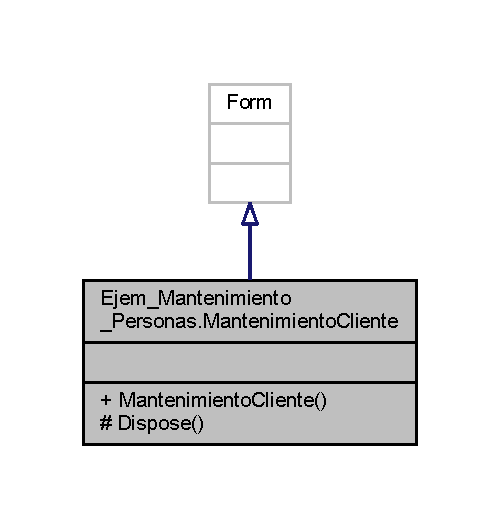
\includegraphics[width=240pt]{class_ejem___mantenimiento___personas_1_1_mantenimiento_cliente__inherit__graph}
\end{center}
\end{figure}


Collaboration diagram for Ejem\+\_\+\+Mantenimiento\+\_\+\+Personas.\+Mantenimiento\+Cliente\+:
\nopagebreak
\begin{figure}[H]
\begin{center}
\leavevmode
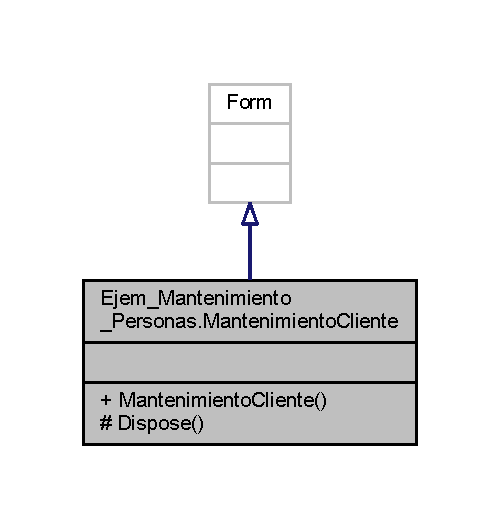
\includegraphics[width=240pt]{class_ejem___mantenimiento___personas_1_1_mantenimiento_cliente__coll__graph}
\end{center}
\end{figure}
\subsection*{Protected Member Functions}
\begin{DoxyCompactItemize}
\item 
override void \mbox{\hyperlink{class_ejem___mantenimiento___personas_1_1_mantenimiento_cliente_a7da653fc99f1760106123912d66f5a5d}{Dispose}} (bool disposing)
\begin{DoxyCompactList}\small\item\em Limpiar los recursos que se estén usando. \end{DoxyCompactList}\end{DoxyCompactItemize}


\subsection{Detailed Description}
Formulario de mantenimiento para los clientes. 



\subsection{Member Function Documentation}
\mbox{\Hypertarget{class_ejem___mantenimiento___personas_1_1_mantenimiento_cliente_a7da653fc99f1760106123912d66f5a5d}\label{class_ejem___mantenimiento___personas_1_1_mantenimiento_cliente_a7da653fc99f1760106123912d66f5a5d}} 
\index{Ejem\+\_\+\+Mantenimiento\+\_\+\+Personas\+::\+Mantenimiento\+Cliente@{Ejem\+\_\+\+Mantenimiento\+\_\+\+Personas\+::\+Mantenimiento\+Cliente}!Dispose@{Dispose}}
\index{Dispose@{Dispose}!Ejem\+\_\+\+Mantenimiento\+\_\+\+Personas\+::\+Mantenimiento\+Cliente@{Ejem\+\_\+\+Mantenimiento\+\_\+\+Personas\+::\+Mantenimiento\+Cliente}}
\subsubsection{\texorpdfstring{Dispose()}{Dispose()}}
{\footnotesize\ttfamily override void Ejem\+\_\+\+Mantenimiento\+\_\+\+Personas.\+Mantenimiento\+Cliente.\+Dispose (\begin{DoxyParamCaption}\item[{bool}]{disposing }\end{DoxyParamCaption})\hspace{0.3cm}{\ttfamily [protected]}}



Limpiar los recursos que se estén usando. 


\begin{DoxyParams}{Parameters}
{\em disposing} & true si los recursos administrados se deben desechar; false en caso contrario.\\
\hline
\end{DoxyParams}


The documentation for this class was generated from the following files\+:\begin{DoxyCompactItemize}
\item 
Mantenimiento\+Cliente.\+cs\item 
Mantenimiento\+Cliente.\+Designer.\+cs\end{DoxyCompactItemize}

%--- End generated contents ---

% Index
\backmatter
\newpage
\phantomsection
\clearemptydoublepage
\addcontentsline{toc}{chapter}{Index}
\printindex

\end{document}
